\documentclass[1p]{elsarticle_modified}
%\bibliographystyle{elsarticle-num}

%\usepackage[colorlinks]{hyperref}
%\usepackage{abbrmath_seonhwa} %\Abb, \Ascr, \Acal ,\Abf, \Afrak
\usepackage{amsfonts}
\usepackage{amssymb}
\usepackage{amsmath}
\usepackage{amsthm}
\usepackage{scalefnt}
\usepackage{amsbsy}
\usepackage{kotex}
\usepackage{caption}
\usepackage{subfig}
\usepackage{color}
\usepackage{graphicx}
\usepackage{xcolor} %% white, black, red, green, blue, cyan, magenta, yellow
\usepackage{float}
\usepackage{setspace}
\usepackage{hyperref}

\usepackage{tikz}
\usetikzlibrary{arrows}

\usepackage{multirow}
\usepackage{array} % fixed length table
\usepackage{hhline}

%%%%%%%%%%%%%%%%%%%%%
\makeatletter
\renewcommand*\env@matrix[1][\arraystretch]{%
	\edef\arraystretch{#1}%
	\hskip -\arraycolsep
	\let\@ifnextchar\new@ifnextchar
	\array{*\c@MaxMatrixCols c}}
\makeatother %https://tex.stackexchange.com/questions/14071/how-can-i-increase-the-line-spacing-in-a-matrix
%%%%%%%%%%%%%%%

\usepackage[normalem]{ulem}

\newcommand{\msout}[1]{\ifmmode\text{\sout{\ensuremath{#1}}}\else\sout{#1}\fi}
%SOURCE: \msout is \stkout macro in https://tex.stackexchange.com/questions/20609/strikeout-in-math-mode

\newcommand{\cancel}[1]{
	\ifmmode
	{\color{red}\msout{#1}}
	\else
	{\color{red}\sout{#1}}
	\fi
}

\newcommand{\add}[1]{
	{\color{blue}\uwave{#1}}
}

\newcommand{\replace}[2]{
	\ifmmode
	{\color{red}\msout{#1}}{\color{blue}\uwave{#2}}
	\else
	{\color{red}\sout{#1}}{\color{blue}\uwave{#2}}
	\fi
}

\newcommand{\Sol}{\mathcal{S}} %segment
\newcommand{\D}{D} %diagram
\newcommand{\A}{\mathcal{A}} %arc


%%%%%%%%%%%%%%%%%%%%%%%%%%%%%5 test

\def\sl{\operatorname{\textup{SL}}(2,\Cbb)}
\def\psl{\operatorname{\textup{PSL}}(2,\Cbb)}
\def\quan{\mkern 1mu \triangleright \mkern 1mu}

\theoremstyle{definition}
\newtheorem{thm}{Theorem}[section]
\newtheorem{prop}[thm]{Proposition}
\newtheorem{lem}[thm]{Lemma}
\newtheorem{ques}[thm]{Question}
\newtheorem{cor}[thm]{Corollary}
\newtheorem{defn}[thm]{Definition}
\newtheorem{exam}[thm]{Example}
\newtheorem{rmk}[thm]{Remark}
\newtheorem{alg}[thm]{Algorithm}

\newcommand{\I}{\sqrt{-1}}
\begin{document}

%\begin{frontmatter}
%
%\title{Boundary parabolic representations of knots up to 8 crossings}
%
%%% Group authors per affiliation:
%\author{Yunhi Cho} 
%\address{Department of Mathematics, University of Seoul, Seoul, Korea}
%\ead{yhcho@uos.ac.kr}
%
%
%\author{Seonhwa Kim} %\fnref{s_kim}}
%\address{Center for Geometry and Physics, Institute for Basic Science, Pohang, 37673, Korea}
%\ead{ryeona17@ibs.re.kr}
%
%\author{Hyuk Kim}
%\address{Department of Mathematical Sciences, Seoul National University, Seoul 08826, Korea}
%\ead{hyukkim@snu.ac.kr}
%
%\author{Seokbeom Yoon}
%\address{Department of Mathematical Sciences, Seoul National University, Seoul, 08826,  Korea}
%\ead{sbyoon15@snu.ac.kr}
%
%\begin{abstract}
%We find all boundary parabolic representation of knots up to 8 crossings.
%
%\end{abstract}
%\begin{keyword}
%    \MSC[2010] 57M25 
%\end{keyword}
%
%\end{frontmatter}

%\linenumbers
%\tableofcontents
%
\newcommand\colored[1]{\textcolor{white}{\rule[-0.35ex]{0.8em}{1.4ex}}\kern-0.8em\color{red} #1}%
%\newcommand\colored[1]{\textcolor{white}{ #1}\kern-2.17ex	\textcolor{white}{ #1}\kern-1.81ex	\textcolor{white}{ #1}\kern-2.15ex\color{red}#1	}

{\Large $\underline{12a_{1164}~(K12a_{1164})}$}

\setlength{\tabcolsep}{10pt}
\renewcommand{\arraystretch}{1.6}
\vspace{1cm}\begin{tabular}{m{100pt}>{\centering\arraybackslash}m{274pt}}
\multirow{5}{120pt}{
	\centering
	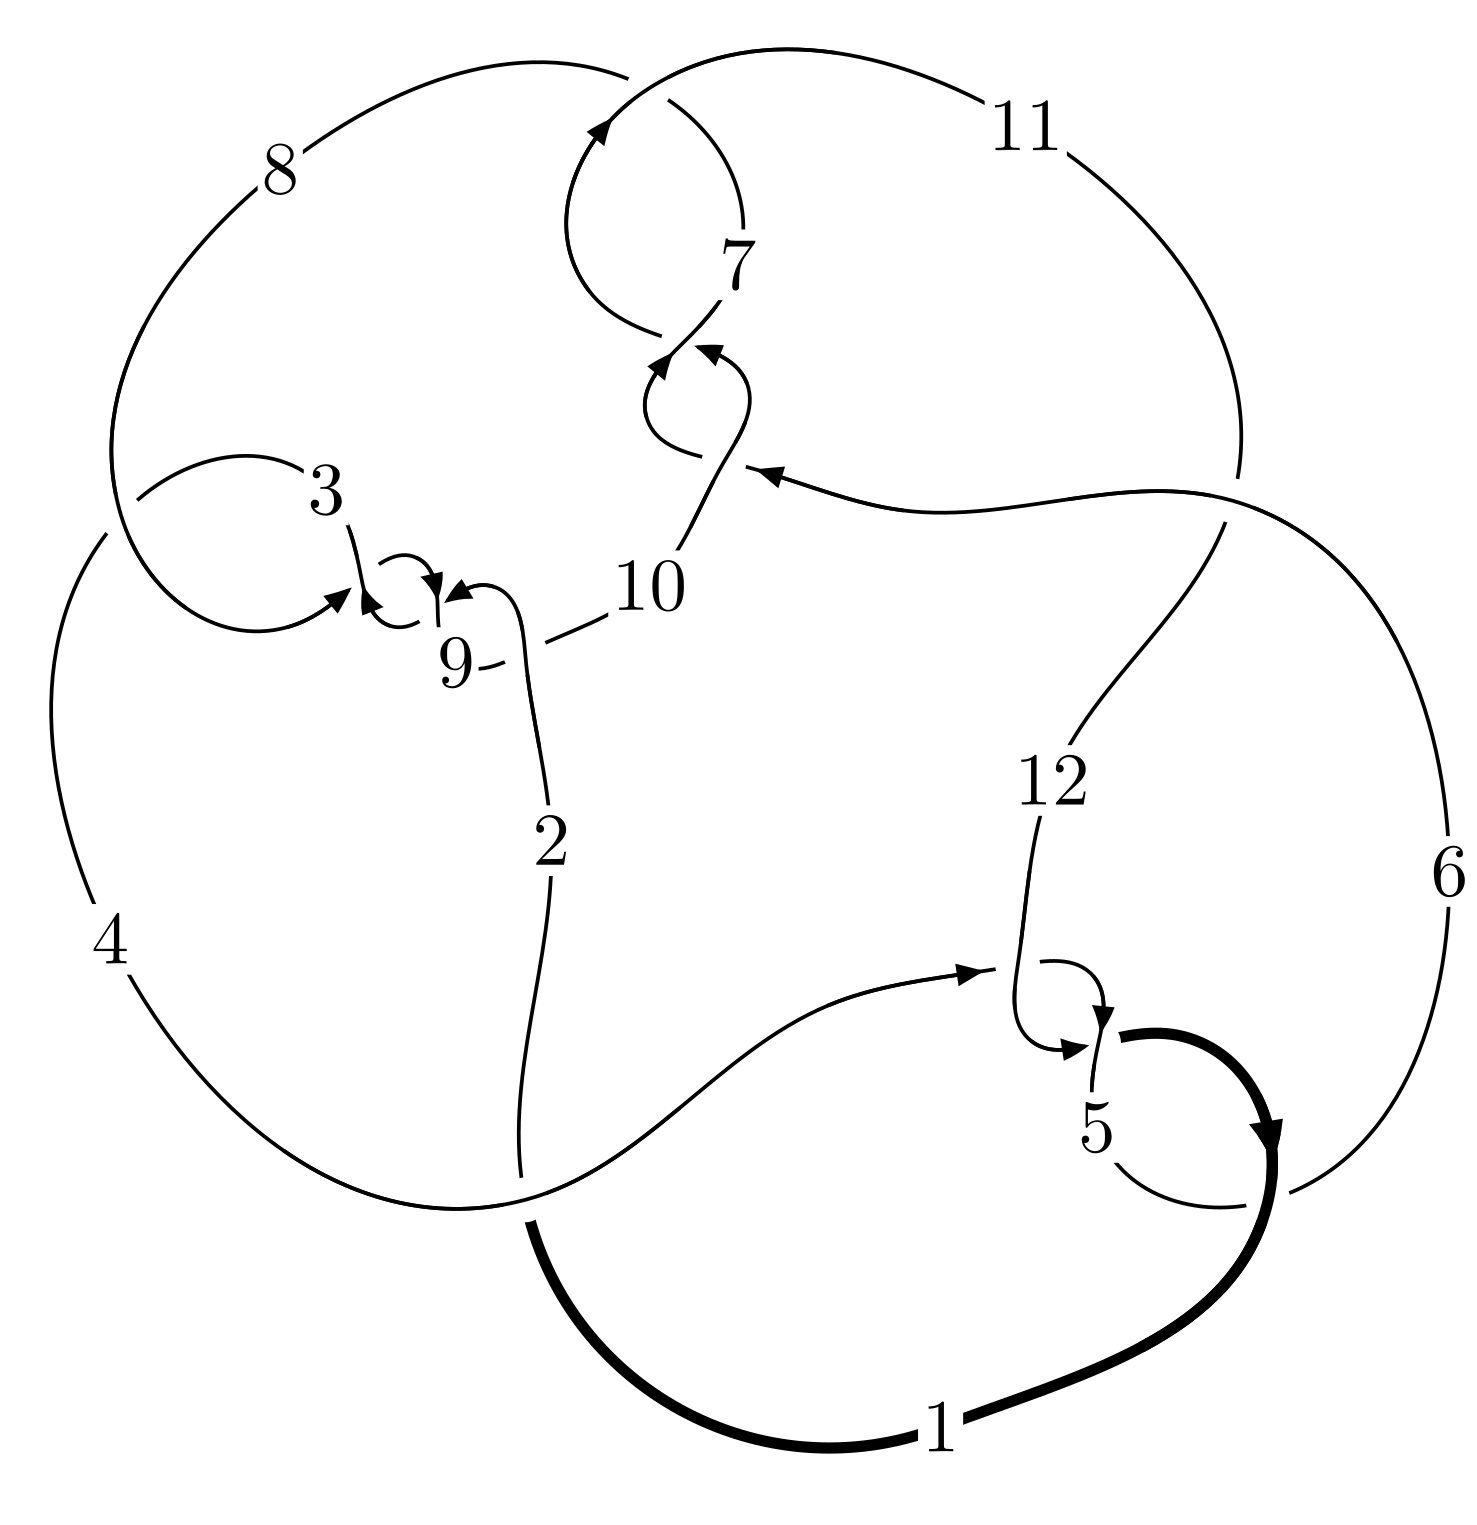
\includegraphics[width=112pt]{../../../GIT/diagram.site/Diagrams/png/1965_12a_1164.png}\\
\ \ \ A knot diagram\footnotemark}&
\allowdisplaybreaks
\textbf{Linearized knot diagam} \\
\cline{2-2}
 &
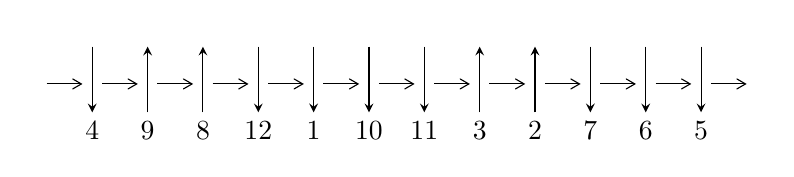
\begin{tikzpicture}[x=20pt, y=17pt]
	% nodes
	\node (C0) at (0, 0) {};
	\node (C1) at (1, 0) {};
	\node (C1U) at (1, +1) {};
	\node (C1D) at (1, -1) {4};

	\node (C2) at (2, 0) {};
	\node (C2U) at (2, +1) {};
	\node (C2D) at (2, -1) {9};

	\node (C3) at (3, 0) {};
	\node (C3U) at (3, +1) {};
	\node (C3D) at (3, -1) {8};

	\node (C4) at (4, 0) {};
	\node (C4U) at (4, +1) {};
	\node (C4D) at (4, -1) {12};

	\node (C5) at (5, 0) {};
	\node (C5U) at (5, +1) {};
	\node (C5D) at (5, -1) {1};

	\node (C6) at (6, 0) {};
	\node (C6U) at (6, +1) {};
	\node (C6D) at (6, -1) {10};

	\node (C7) at (7, 0) {};
	\node (C7U) at (7, +1) {};
	\node (C7D) at (7, -1) {11};

	\node (C8) at (8, 0) {};
	\node (C8U) at (8, +1) {};
	\node (C8D) at (8, -1) {3};

	\node (C9) at (9, 0) {};
	\node (C9U) at (9, +1) {};
	\node (C9D) at (9, -1) {2};

	\node (C10) at (10, 0) {};
	\node (C10U) at (10, +1) {};
	\node (C10D) at (10, -1) {7};

	\node (C11) at (11, 0) {};
	\node (C11U) at (11, +1) {};
	\node (C11D) at (11, -1) {6};

	\node (C12) at (12, 0) {};
	\node (C12U) at (12, +1) {};
	\node (C12D) at (12, -1) {5};
	\node (C13) at (13, 0) {};

	% arrows
	\draw[->,>={angle 60}]
	(C0) edge (C1) (C1) edge (C2) (C2) edge (C3) (C3) edge (C4) (C4) edge (C5) (C5) edge (C6) (C6) edge (C7) (C7) edge (C8) (C8) edge (C9) (C9) edge (C10) (C10) edge (C11) (C11) edge (C12) (C12) edge (C13) ;	\draw[->,>=stealth]
	(C1U) edge (C1D) (C2D) edge (C2U) (C3D) edge (C3U) (C4U) edge (C4D) (C5U) edge (C5D) (C6U) edge (C6D) (C7U) edge (C7D) (C8D) edge (C8U) (C9D) edge (C9U) (C10U) edge (C10D) (C11U) edge (C11D) (C12U) edge (C12D) ;
	\end{tikzpicture} \\
\hhline{~~} \\& 
\textbf{Solving Sequence} \\ \cline{2-2} 
 &
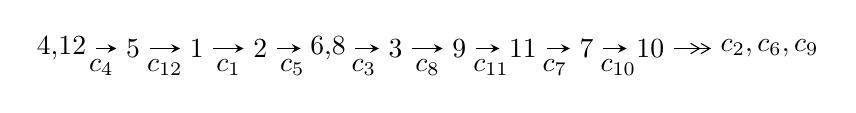
\begin{tikzpicture}[x=23pt, y=7pt]
	% node
	\node (A0) at (-1/8, 0) {4,12};
	\node (A1) at (1, 0) {5};
	\node (A2) at (2, 0) {1};
	\node (A3) at (3, 0) {2};
	\node (A4) at (65/16, 0) {6,8};
	\node (A5) at (41/8, 0) {3};
	\node (A6) at (49/8, 0) {9};
	\node (A7) at (57/8, 0) {11};
	\node (A8) at (65/8, 0) {7};
	\node (A9) at (73/8, 0) {10};
	\node (C1) at (1/2, -1) {$c_{4}$};
	\node (C2) at (3/2, -1) {$c_{12}$};
	\node (C3) at (5/2, -1) {$c_{1}$};
	\node (C4) at (7/2, -1) {$c_{5}$};
	\node (C5) at (37/8, -1) {$c_{3}$};
	\node (C6) at (45/8, -1) {$c_{8}$};
	\node (C7) at (53/8, -1) {$c_{11}$};
	\node (C8) at (61/8, -1) {$c_{7}$};
	\node (C9) at (69/8, -1) {$c_{10}$};
	\node (A10) at (11, 0) {$c_{2},c_{6},c_{9}$};

	% edge
	\draw[->,>=stealth]	
	(A0) edge (A1) (A1) edge (A2) (A2) edge (A3) (A3) edge (A4) (A4) edge (A5) (A5) edge (A6) (A6) edge (A7) (A7) edge (A8) (A8) edge (A9) ;
	\draw[->>,>={angle 60}]	
	(A9) edge (A10);
\end{tikzpicture} \\ 

\end{tabular} \\

\footnotetext{
The image of knot diagram is generated by the software ``\textbf{Draw programme}" developed by Andrew Bartholomew(\url{http://www.layer8.co.uk/maths/draw/index.htm\#Running-draw}), where we modified some parts for our purpose(\url{https://github.com/CATsTAILs/LinksPainter}).
}\phantom \\ \newline 
\centering \textbf{Ideals for irreducible components\footnotemark of $X_{\text{par}}$} 
 
\begin{align*}
I^u_{1}&=\langle 
u^{19}+u^{18}+\cdots+2 b-1,\;u^6-3 u^4+2 u^2+a+1,\;u^{21}+u^{20}+\cdots+u+1\rangle \\
I^u_{2}&=\langle 
-1056266 u^{33}-534744 u^{32}+\cdots+2309809 b-234638,\\
\phantom{I^u_{2}}&\phantom{= \langle  }-619436 u^{33}-841682 u^{32}+\cdots+6929427 a-2733846,\;u^{34}+u^{33}+\cdots+6 u-3\rangle \\
I^u_{3}&=\langle 
b^2+2,\;a+1,\;u-1\rangle \\
I^u_{4}&=\langle 
b,\;a+1,\;u+1\rangle \\
\\
\end{align*}
\raggedright * 4 irreducible components of $\dim_{\mathbb{C}}=0$, with total 58 representations.\\
\footnotetext{All coefficients of polynomials are rational numbers. But the coefficients are sometimes approximated in decimal forms when there is not enough margin.}
\newpage
\renewcommand{\arraystretch}{1}
\centering \section*{I. $I^u_{1}= \langle u^{19}+u^{18}+\cdots+2 b-1,\;u^6-3 u^4+2 u^2+a+1,\;u^{21}+u^{20}+\cdots+u+1 \rangle$}
\flushleft \textbf{(i) Arc colorings}\\
\begin{tabular}{m{7pt} m{180pt} m{7pt} m{180pt} }
\flushright $a_{4}=$&$\begin{pmatrix}1\\0\end{pmatrix}$ \\
\flushright $a_{12}=$&$\begin{pmatrix}0\\u\end{pmatrix}$ \\
\flushright $a_{5}=$&$\begin{pmatrix}1\\u^2\end{pmatrix}$ \\
\flushright $a_{1}=$&$\begin{pmatrix}- u\\- u^3+u\end{pmatrix}$ \\
\flushright $a_{2}=$&$\begin{pmatrix}u^3-2 u\\- u^3+u\end{pmatrix}$ \\
\flushright $a_{6}=$&$\begin{pmatrix}- u^2+1\\- u^4+2 u^2\end{pmatrix}$ \\
\flushright $a_{8}=$&$\begin{pmatrix}- u^6+3 u^4-2 u^2-1\\-\frac{1}{2} u^{19}-\frac{1}{2} u^{18}+\cdots+\frac{1}{2} u+\frac{1}{2}\end{pmatrix}$ \\
\flushright $a_{3}=$&$\begin{pmatrix}\frac{1}{2} u^{19}+\frac{1}{2} u^{18}+\cdots-\frac{1}{2} u+\frac{1}{2}\\\frac{1}{2} u^{20}-5 u^{18}+\cdots- u-\frac{1}{2}\end{pmatrix}$ \\
\flushright $a_{9}=$&$\begin{pmatrix}-\frac{1}{2} u^{20}-\frac{1}{2} u^{19}+\cdots+\frac{1}{2} u^2+\frac{5}{2} u\\\frac{1}{2} u^{20}+\frac{1}{2} u^{19}+\cdots-\frac{1}{2} u^2+\frac{1}{2} u\end{pmatrix}$ \\
\flushright $a_{11}=$&$\begin{pmatrix}u^5-2 u^3+u\\u^7-3 u^5+2 u^3+u\end{pmatrix}$ \\
\flushright $a_{7}=$&$\begin{pmatrix}u^4- u^2-1\\-\frac{1}{2} u^{19}-\frac{1}{2} u^{18}+\cdots+\frac{1}{2} u+\frac{1}{2}\end{pmatrix}$ \\
\flushright $a_{10}=$&$\begin{pmatrix}- u^3+2 u\\\frac{1}{2} u^{20}+\frac{1}{2} u^{19}+\cdots-\frac{1}{2} u^2+\frac{1}{2} u\end{pmatrix}$\\&\end{tabular}
\flushleft \textbf{(ii) Obstruction class $= -1$}\\~\\
\flushleft \textbf{(iii) Cusp Shapes $= - u^{20}+u^{19}+13 u^{18}-10 u^{17}-67 u^{16}+44 u^{15}+175 u^{14}-107 u^{13}-225 u^{12}+145 u^{11}+63 u^{10}-83 u^9+168 u^8-36 u^7-146 u^6+70 u^5-25 u^4-11 u^3+41 u^2-17 u-6$}\\~\\
\newpage\renewcommand{\arraystretch}{1}
\flushleft \textbf{(iv) u-Polynomials at the component}\newline \\
\begin{tabular}{m{50pt}|m{274pt}}
Crossings & \hspace{64pt}u-Polynomials at each crossing \\
\hline $$\begin{aligned}c_{1},c_{11}\end{aligned}$$&$\begin{aligned}
&u^{21}-3 u^{20}+\cdots+16 u^2-16
\end{aligned}$\\
\hline $$\begin{aligned}c_{2},c_{3},c_{8}\\c_{9}\end{aligned}$$&$\begin{aligned}
&u^{21}+3 u^{20}+\cdots-4 u-2
\end{aligned}$\\
\hline $$\begin{aligned}c_{4},c_{5},c_{6}\\c_{7},c_{10},c_{12}\end{aligned}$$&$\begin{aligned}
&u^{21}+u^{20}+\cdots+u+1
\end{aligned}$\\
\hline
\end{tabular}\\~\\
\newpage\renewcommand{\arraystretch}{1}
\flushleft \textbf{(v) Riley Polynomials at the component}\newline \\
\begin{tabular}{m{50pt}|m{274pt}}
Crossings & \hspace{64pt}Riley Polynomials at each crossing \\
\hline $$\begin{aligned}c_{1},c_{11}\end{aligned}$$&$\begin{aligned}
&y^{21}+11 y^{20}+\cdots+512 y-256
\end{aligned}$\\
\hline $$\begin{aligned}c_{2},c_{3},c_{8}\\c_{9}\end{aligned}$$&$\begin{aligned}
&y^{21}+23 y^{20}+\cdots-32 y-4
\end{aligned}$\\
\hline $$\begin{aligned}c_{4},c_{5},c_{6}\\c_{7},c_{10},c_{12}\end{aligned}$$&$\begin{aligned}
&y^{21}-21 y^{20}+\cdots-3 y-1
\end{aligned}$\\
\hline
\end{tabular}\\~\\
\newpage\flushleft \textbf{(vi) Complex Volumes and Cusp Shapes}
$$\begin{array}{c|c|c}  
\text{Solutions to }I^u_{1}& \I (\text{vol} + \sqrt{-1}CS) & \text{Cusp shape}\\
 \hline 
\begin{aligned}
u &= \phantom{-}0.121015 + 0.802604 I \\
a &= \phantom{-}1.51299 - 1.34586 I \\
b &= -0.16702 + 1.51542 I\end{aligned}
 & -2.09551 - 4.69375 I & -3.63503 + 3.84735 I \\ \hline\begin{aligned}
u &= \phantom{-}0.121015 - 0.802604 I \\
a &= \phantom{-}1.51299 + 1.34586 I \\
b &= -0.16702 - 1.51542 I\end{aligned}
 & -2.09551 + 4.69375 I & -3.63503 - 3.84735 I \\ \hline\begin{aligned}
u &= -0.040007 + 0.789380 I \\
a &= \phantom{-}1.62258 + 0.43481 I \\
b &= -0.588267 - 0.491565 I\end{aligned}
 & \phantom{-}4.51526 + 2.01021 I & \phantom{-}0.41448 - 3.78371 I \\ \hline\begin{aligned}
u &= -0.040007 - 0.789380 I \\
a &= \phantom{-}1.62258 - 0.43481 I \\
b &= -0.588267 + 0.491565 I\end{aligned}
 & \phantom{-}4.51526 - 2.01021 I & \phantom{-}0.41448 + 3.78371 I \\ \hline\begin{aligned}
u &= \phantom{-}1.283400 + 0.250591 I \\
a &= \phantom{-}0.110044 + 0.250523 I \\
b &= -0.205916 - 1.377950 I\end{aligned}
 & -9.03034 - 2.72457 I & -12.33705 + 3.20097 I \\ \hline\begin{aligned}
u &= \phantom{-}1.283400 - 0.250591 I \\
a &= \phantom{-}0.110044 - 0.250523 I \\
b &= -0.205916 + 1.377950 I\end{aligned}
 & -9.03034 + 2.72457 I & -12.33705 - 3.20097 I \\ \hline\begin{aligned}
u &= -1.35078\phantom{ +0.000000I} \\
a &= -0.736116\phantom{ +0.000000I} \\
b &= \phantom{-}0.673734\phantom{ +0.000000I}\end{aligned}
 & -7.60400\phantom{ +0.000000I} & -10.4800\phantom{ +0.000000I} \\ \hline\begin{aligned}
u &= -1.319980 + 0.321329 I \\
a &= \phantom{-}0.757736 - 0.419310 I \\
b &= -0.688597 + 0.357279 I\end{aligned}
 & -3.53789 + 5.93688 I & -7.80246 - 3.12775 I \\ \hline\begin{aligned}
u &= -1.319980 - 0.321329 I \\
a &= \phantom{-}0.757736 + 0.419310 I \\
b &= -0.688597 - 0.357279 I\end{aligned}
 & -3.53789 - 5.93688 I & -7.80246 + 3.12775 I \\ \hline\begin{aligned}
u &= \phantom{-}1.388650 + 0.093259 I \\
a &= -0.673057 - 0.380782 I \\
b &= \phantom{-}0.353596 - 0.874613 I\end{aligned}
 & -10.38940 - 3.55849 I & -14.4570 + 4.3859 I\\
 \hline 
 \end{array}$$\newpage$$\begin{array}{c|c|c}  
\text{Solutions to }I^u_{1}& \I (\text{vol} + \sqrt{-1}CS) & \text{Cusp shape}\\
 \hline 
\begin{aligned}
u &= \phantom{-}1.388650 - 0.093259 I \\
a &= -0.673057 + 0.380782 I \\
b &= \phantom{-}0.353596 + 0.874613 I\end{aligned}
 & -10.38940 + 3.55849 I & -14.4570 - 4.3859 I \\ \hline\begin{aligned}
u &= \phantom{-}1.353780 + 0.356484 I \\
a &= \phantom{-}1.326430 + 0.422608 I \\
b &= -0.624029 + 0.625071 I\end{aligned}
 & -4.33607 - 10.34760 I & -9.08482 + 8.30410 I \\ \hline\begin{aligned}
u &= \phantom{-}1.353780 - 0.356484 I \\
a &= \phantom{-}1.326430 - 0.422608 I \\
b &= -0.624029 - 0.625071 I\end{aligned}
 & -4.33607 + 10.34760 I & -9.08482 - 8.30410 I \\ \hline\begin{aligned}
u &= -1.38701 + 0.37866 I \\
a &= \phantom{-}1.88840 - 0.29011 I \\
b &= -0.19424 - 1.57233 I\end{aligned}
 & -11.6562 + 13.3679 I & -11.96534 - 7.27527 I \\ \hline\begin{aligned}
u &= -1.38701 - 0.37866 I \\
a &= \phantom{-}1.88840 + 0.29011 I \\
b &= -0.19424 + 1.57233 I\end{aligned}
 & -11.6562 - 13.3679 I & -11.96534 + 7.27527 I \\ \hline\begin{aligned}
u &= \phantom{-}0.445437 + 0.325177 I \\
a &= -1.38881 - 0.40146 I \\
b &= \phantom{-}0.02269 - 1.49213 I\end{aligned}
 & -6.40486 - 1.31691 I & -7.01863 + 5.01587 I \\ \hline\begin{aligned}
u &= \phantom{-}0.445437 - 0.325177 I \\
a &= -1.38881 + 0.40146 I \\
b &= \phantom{-}0.02269 + 1.49213 I\end{aligned}
 & -6.40486 + 1.31691 I & -7.01863 - 5.01587 I \\ \hline\begin{aligned}
u &= -1.47176 + 0.13523 I \\
a &= -0.818744 + 1.112050 I \\
b &= \phantom{-}0.06951 + 1.62601 I\end{aligned}
 & -18.9337 + 4.9859 I & -15.7556 - 3.2060 I \\ \hline\begin{aligned}
u &= -1.47176 - 0.13523 I \\
a &= -0.818744 - 1.112050 I \\
b &= \phantom{-}0.06951 - 1.62601 I\end{aligned}
 & -18.9337 - 4.9859 I & -15.7556 + 3.2060 I \\ \hline\begin{aligned}
u &= -0.198124 + 0.264706 I \\
a &= -0.969512 + 0.228317 I \\
b &= \phantom{-}0.185405 + 0.382871 I\end{aligned}
 & -0.126670 + 0.730510 I & -4.11837 - 9.53132 I\\
 \hline 
 \end{array}$$\newpage$$\begin{array}{c|c|c}  
\text{Solutions to }I^u_{1}& \I (\text{vol} + \sqrt{-1}CS) & \text{Cusp shape}\\
 \hline 
\begin{aligned}
u &= -0.198124 - 0.264706 I \\
a &= -0.969512 - 0.228317 I \\
b &= \phantom{-}0.185405 - 0.382871 I\end{aligned}
 & -0.126670 - 0.730510 I & -4.11837 + 9.53132 I\\
 \hline 
 \end{array}$$\newpage\newpage\renewcommand{\arraystretch}{1}
\centering \section*{II. $I^u_{2}= \langle -1.06\times10^{6} u^{33}-5.35\times10^{5} u^{32}+\cdots+2.31\times10^{6} b-2.35\times10^{5},\;-6.19\times10^{5} u^{33}-8.42\times10^{5} u^{32}+\cdots+6.93\times10^{6} a-2.73\times10^{6},\;u^{34}+u^{33}+\cdots+6 u-3 \rangle$}
\flushleft \textbf{(i) Arc colorings}\\
\begin{tabular}{m{7pt} m{180pt} m{7pt} m{180pt} }
\flushright $a_{4}=$&$\begin{pmatrix}1\\0\end{pmatrix}$ \\
\flushright $a_{12}=$&$\begin{pmatrix}0\\u\end{pmatrix}$ \\
\flushright $a_{5}=$&$\begin{pmatrix}1\\u^2\end{pmatrix}$ \\
\flushright $a_{1}=$&$\begin{pmatrix}- u\\- u^3+u\end{pmatrix}$ \\
\flushright $a_{2}=$&$\begin{pmatrix}u^3-2 u\\- u^3+u\end{pmatrix}$ \\
\flushright $a_{6}=$&$\begin{pmatrix}- u^2+1\\- u^4+2 u^2\end{pmatrix}$ \\
\flushright $a_{8}=$&$\begin{pmatrix}0.0893921 u^{33}+0.121465 u^{32}+\cdots+3.10263 u+0.394527\\0.457296 u^{33}+0.231510 u^{32}+\cdots-1.08414 u+0.101583\end{pmatrix}$ \\
\flushright $a_{3}=$&$\begin{pmatrix}-0.408040 u^{33}-0.237636 u^{32}+\cdots+4.75198 u-0.453759\\-0.180498 u^{33}+0.325687 u^{32}+\cdots-2.48353 u+0.264153\end{pmatrix}$ \\
\flushright $a_{9}=$&$\begin{pmatrix}-0.0764438 u^{33}-0.0671149 u^{32}+\cdots-1.96468 u+3.75923\\-0.151130 u^{33}-0.0265009 u^{32}+\cdots+1.29755 u-1.23819\end{pmatrix}$ \\
\flushright $a_{11}=$&$\begin{pmatrix}u^5-2 u^3+u\\u^7-3 u^5+2 u^3+u\end{pmatrix}$ \\
\flushright $a_{7}=$&$\begin{pmatrix}-0.328926 u^{33}-0.0100975 u^{32}+\cdots+5.68192 u-0.510619\\0.418318 u^{33}+0.131562 u^{32}+\cdots-2.57929 u-0.0948537\end{pmatrix}$ \\
\flushright $a_{10}=$&$\begin{pmatrix}0.350446 u^{33}+0.00787828 u^{32}+\cdots+1.10883 u+1.78222\\-0.352234 u^{33}-0.131296 u^{32}+\cdots+0.866235 u-0.633064\end{pmatrix}$\\&\end{tabular}
\flushleft \textbf{(ii) Obstruction class $= -1$}\\~\\
\flushleft \textbf{(iii) Cusp Shapes $= \frac{113576}{2309809} u^{33}+\frac{5887808}{2309809} u^{32}+\cdots-\frac{11535388}{2309809} u-\frac{230526}{2309809}$}\\~\\
\newpage\renewcommand{\arraystretch}{1}
\flushleft \textbf{(iv) u-Polynomials at the component}\newline \\
\begin{tabular}{m{50pt}|m{274pt}}
Crossings & \hspace{64pt}u-Polynomials at each crossing \\
\hline $$\begin{aligned}c_{1},c_{11}\end{aligned}$$&$\begin{aligned}
&(u^{17}-3 u^{16}+\cdots+9 u-3)^{2}
\end{aligned}$\\
\hline $$\begin{aligned}c_{2},c_{3},c_{8}\\c_{9}\end{aligned}$$&$\begin{aligned}
&(u^{17}- u^{16}+\cdots+u+1)^{2}
\end{aligned}$\\
\hline $$\begin{aligned}c_{4},c_{5},c_{6}\\c_{7},c_{10},c_{12}\end{aligned}$$&$\begin{aligned}
&u^{34}+u^{33}+\cdots+6 u-3
\end{aligned}$\\
\hline
\end{tabular}\\~\\
\newpage\renewcommand{\arraystretch}{1}
\flushleft \textbf{(v) Riley Polynomials at the component}\newline \\
\begin{tabular}{m{50pt}|m{274pt}}
Crossings & \hspace{64pt}Riley Polynomials at each crossing \\
\hline $$\begin{aligned}c_{1},c_{11}\end{aligned}$$&$\begin{aligned}
&(y^{17}+11 y^{16}+\cdots+57 y-9)^{2}
\end{aligned}$\\
\hline $$\begin{aligned}c_{2},c_{3},c_{8}\\c_{9}\end{aligned}$$&$\begin{aligned}
&(y^{17}+19 y^{16}+\cdots+y-1)^{2}
\end{aligned}$\\
\hline $$\begin{aligned}c_{4},c_{5},c_{6}\\c_{7},c_{10},c_{12}\end{aligned}$$&$\begin{aligned}
&y^{34}-25 y^{33}+\cdots-48 y+9
\end{aligned}$\\
\hline
\end{tabular}\\~\\
\newpage\flushleft \textbf{(vi) Complex Volumes and Cusp Shapes}
$$\begin{array}{c|c|c}  
\text{Solutions to }I^u_{2}& \I (\text{vol} + \sqrt{-1}CS) & \text{Cusp shape}\\
 \hline 
\begin{aligned}
u &= \phantom{-}0.180995 + 0.883653 I \\
a &= -1.35621 + 1.29271 I \\
b &= \phantom{-}0.17426 - 1.55100 I\end{aligned}
 & -6.70220 - 8.83664 I & -8.37368 + 5.87120 I \\ \hline\begin{aligned}
u &= \phantom{-}0.180995 - 0.883653 I \\
a &= -1.35621 - 1.29271 I \\
b &= \phantom{-}0.17426 + 1.55100 I\end{aligned}
 & -6.70220 + 8.83664 I & -8.37368 - 5.87120 I \\ \hline\begin{aligned}
u &= \phantom{-}0.595797 + 0.672047 I \\
a &= \phantom{-}0.993055 - 0.599481 I \\
b &= -0.02780 + 1.57600 I\end{aligned}
 & -12.06090 - 2.39923 I & -12.86600 + 3.27109 I \\ \hline\begin{aligned}
u &= \phantom{-}0.595797 - 0.672047 I \\
a &= \phantom{-}0.993055 + 0.599481 I \\
b &= -0.02780 - 1.57600 I\end{aligned}
 & -12.06090 + 2.39923 I & -12.86600 - 3.27109 I \\ \hline\begin{aligned}
u &= -1.13369\phantom{ +0.000000I} \\
a &= \phantom{-}0.407824\phantom{ +0.000000I} \\
b &= -0.387802\phantom{ +0.000000I}\end{aligned}
 & -2.28510\phantom{ +0.000000I} & -1.13090\phantom{ +0.000000I} \\ \hline\begin{aligned}
u &= -0.136716 + 0.824881 I \\
a &= -1.58020 - 0.51459 I \\
b &= \phantom{-}0.580614 + 0.569922 I\end{aligned}
 & \phantom{-}0.35577 + 6.09306 I & -4.70703 - 6.87425 I \\ \hline\begin{aligned}
u &= -0.136716 - 0.824881 I \\
a &= -1.58020 + 0.51459 I \\
b &= \phantom{-}0.580614 - 0.569922 I\end{aligned}
 & \phantom{-}0.35577 - 6.09306 I & -4.70703 + 6.87425 I \\ \hline\begin{aligned}
u &= -1.101130 + 0.389395 I \\
a &= \phantom{-}0.509094 - 0.606456 I \\
b &= -0.488571 + 0.501958 I\end{aligned}
 & -2.59185 - 1.70542 I & -7.89077 + 4.02096 I \\ \hline\begin{aligned}
u &= -1.101130 - 0.389395 I \\
a &= \phantom{-}0.509094 + 0.606456 I \\
b &= -0.488571 - 0.501958 I\end{aligned}
 & -2.59185 + 1.70542 I & -7.89077 - 4.02096 I \\ \hline\begin{aligned}
u &= \phantom{-}1.128290 + 0.347386 I \\
a &= \phantom{-}0.098642 - 0.298753 I \\
b &= \phantom{-}0.14171 + 1.46572 I\end{aligned}
 & -5.15765 + 0.50801 I & -6.42549 + 0.23246 I\\
 \hline 
 \end{array}$$\newpage$$\begin{array}{c|c|c}  
\text{Solutions to }I^u_{2}& \I (\text{vol} + \sqrt{-1}CS) & \text{Cusp shape}\\
 \hline 
\begin{aligned}
u &= \phantom{-}1.128290 - 0.347386 I \\
a &= \phantom{-}0.098642 + 0.298753 I \\
b &= \phantom{-}0.14171 - 1.46572 I\end{aligned}
 & -5.15765 - 0.50801 I & -6.42549 - 0.23246 I \\ \hline\begin{aligned}
u &= \phantom{-}1.080650 + 0.504832 I \\
a &= -0.224516 + 0.457220 I \\
b &= -0.13662 - 1.53895 I\end{aligned}
 & -9.44087 + 3.91820 I & -11.59784 - 2.39256 I \\ \hline\begin{aligned}
u &= \phantom{-}1.080650 - 0.504832 I \\
a &= -0.224516 - 0.457220 I \\
b &= -0.13662 + 1.53895 I\end{aligned}
 & -9.44087 - 3.91820 I & -11.59784 + 2.39256 I \\ \hline\begin{aligned}
u &= \phantom{-}0.078456 + 0.750182 I \\
a &= -1.69151 - 0.36066 I \\
b &= \phantom{-}0.601563 + 0.400803 I\end{aligned}
 & \phantom{-}0.85249 - 2.05778 I & -2.98070 + 0.37816 I \\ \hline\begin{aligned}
u &= \phantom{-}0.078456 - 0.750182 I \\
a &= -1.69151 + 0.36066 I \\
b &= \phantom{-}0.601563 - 0.400803 I\end{aligned}
 & \phantom{-}0.85249 + 2.05778 I & -2.98070 - 0.37816 I \\ \hline\begin{aligned}
u &= \phantom{-}1.213590 + 0.290321 I \\
a &= \phantom{-}1.38485 + 0.75199 I \\
b &= -0.488571 + 0.501958 I\end{aligned}
 & -2.59185 - 1.70542 I & -7.89077 + 4.02096 I \\ \hline\begin{aligned}
u &= \phantom{-}1.213590 - 0.290321 I \\
a &= \phantom{-}1.38485 - 0.75199 I \\
b &= -0.488571 - 0.501958 I\end{aligned}
 & -2.59185 + 1.70542 I & -7.89077 - 4.02096 I \\ \hline\begin{aligned}
u &= \phantom{-}1.260460 + 0.061296 I \\
a &= \phantom{-}0.428262 + 0.963327 I \\
b &= -0.151255 + 0.679822 I\end{aligned}
 & -4.41315 - 1.83062 I & -11.59303 + 5.22267 I \\ \hline\begin{aligned}
u &= \phantom{-}1.260460 - 0.061296 I \\
a &= \phantom{-}0.428262 - 0.963327 I \\
b &= -0.151255 - 0.679822 I\end{aligned}
 & -4.41315 + 1.83062 I & -11.59303 - 5.22267 I \\ \hline\begin{aligned}
u &= -1.230380 + 0.338033 I \\
a &= -0.652848 + 0.475134 I \\
b &= \phantom{-}0.601563 - 0.400803 I\end{aligned}
 & \phantom{-}0.85249 + 2.05778 I & -2.98070 - 0.37816 I\\
 \hline 
 \end{array}$$\newpage$$\begin{array}{c|c|c}  
\text{Solutions to }I^u_{2}& \I (\text{vol} + \sqrt{-1}CS) & \text{Cusp shape}\\
 \hline 
\begin{aligned}
u &= -1.230380 - 0.338033 I \\
a &= -0.652848 - 0.475134 I \\
b &= \phantom{-}0.601563 + 0.400803 I\end{aligned}
 & \phantom{-}0.85249 - 2.05778 I & -2.98070 + 0.37816 I \\ \hline\begin{aligned}
u &= -0.502282 + 0.483544 I \\
a &= \phantom{-}0.782134 + 0.681918 I \\
b &= -0.151255 - 0.679822 I\end{aligned}
 & -4.41315 + 1.83062 I & -11.59303 - 5.22267 I \\ \hline\begin{aligned}
u &= -0.502282 - 0.483544 I \\
a &= \phantom{-}0.782134 - 0.681918 I \\
b &= -0.151255 + 0.679822 I\end{aligned}
 & -4.41315 - 1.83062 I & -11.59303 + 5.22267 I \\ \hline\begin{aligned}
u &= \phantom{-}1.293540 + 0.343405 I \\
a &= -1.35895 - 0.53387 I \\
b &= \phantom{-}0.580614 - 0.569922 I\end{aligned}
 & \phantom{-}0.35577 - 6.09306 I & -4.70703 + 6.87425 I \\ \hline\begin{aligned}
u &= \phantom{-}1.293540 - 0.343405 I \\
a &= -1.35895 + 0.53387 I \\
b &= \phantom{-}0.580614 + 0.569922 I\end{aligned}
 & \phantom{-}0.35577 + 6.09306 I & -4.70703 - 6.87425 I \\ \hline\begin{aligned}
u &= \phantom{-}0.043766 + 0.657258 I \\
a &= -1.87701 + 1.49405 I \\
b &= \phantom{-}0.14171 - 1.46572 I\end{aligned}
 & -5.15765 - 0.50801 I & -6.42549 - 0.23246 I \\ \hline\begin{aligned}
u &= \phantom{-}0.043766 - 0.657258 I \\
a &= -1.87701 - 1.49405 I \\
b &= \phantom{-}0.14171 + 1.46572 I\end{aligned}
 & -5.15765 + 0.50801 I & -6.42549 + 0.23246 I \\ \hline\begin{aligned}
u &= -1.312420 + 0.277525 I \\
a &= \phantom{-}2.25755 - 0.93271 I \\
b &= -0.13662 - 1.53895 I\end{aligned}
 & -9.44087 + 3.91820 I & -11.59784 - 2.39256 I \\ \hline\begin{aligned}
u &= -1.312420 - 0.277525 I \\
a &= \phantom{-}2.25755 + 0.93271 I \\
b &= -0.13662 + 1.53895 I\end{aligned}
 & -9.44087 - 3.91820 I & -11.59784 + 2.39256 I \\ \hline\begin{aligned}
u &= -1.370680 + 0.056095 I \\
a &= \phantom{-}0.56793 - 2.07715 I \\
b &= -0.02780 - 1.57600 I\end{aligned}
 & -12.06090 + 2.39923 I & -12.86600 - 3.27109 I\\
 \hline 
 \end{array}$$\newpage$$\begin{array}{c|c|c}  
\text{Solutions to }I^u_{2}& \I (\text{vol} + \sqrt{-1}CS) & \text{Cusp shape}\\
 \hline 
\begin{aligned}
u &= -1.370680 - 0.056095 I \\
a &= \phantom{-}0.56793 + 2.07715 I \\
b &= -0.02780 + 1.57600 I\end{aligned}
 & -12.06090 - 2.39923 I & -12.86600 + 3.27109 I \\ \hline\begin{aligned}
u &= -1.343580 + 0.346101 I \\
a &= -2.09386 + 0.46604 I \\
b &= \phantom{-}0.17426 + 1.55100 I\end{aligned}
 & -6.70220 + 8.83664 I & -8.37368 - 5.87120 I \\ \hline\begin{aligned}
u &= -1.343580 - 0.346101 I \\
a &= -2.09386 - 0.46604 I \\
b &= \phantom{-}0.17426 - 1.55100 I\end{aligned}
 & -6.70220 - 8.83664 I & -8.37368 + 5.87120 I \\ \hline\begin{aligned}
u &= \phantom{-}0.376966\phantom{ +0.000000I} \\
a &= \phantom{-}2.21933\phantom{ +0.000000I} \\
b &= -0.387802\phantom{ +0.000000I}\end{aligned}
 & -2.28510\phantom{ +0.000000I} & -1.13090\phantom{ +0.000000I}\\
 \hline 
 \end{array}$$\newpage\newpage\renewcommand{\arraystretch}{1}
\centering \section*{III. $I^u_{3}= \langle b^2+2,\;a+1,\;u-1 \rangle$}
\flushleft \textbf{(i) Arc colorings}\\
\begin{tabular}{m{7pt} m{180pt} m{7pt} m{180pt} }
\flushright $a_{4}=$&$\begin{pmatrix}1\\0\end{pmatrix}$ \\
\flushright $a_{12}=$&$\begin{pmatrix}0\\1\end{pmatrix}$ \\
\flushright $a_{5}=$&$\begin{pmatrix}1\\1\end{pmatrix}$ \\
\flushright $a_{1}=$&$\begin{pmatrix}-1\\0\end{pmatrix}$ \\
\flushright $a_{2}=$&$\begin{pmatrix}-1\\0\end{pmatrix}$ \\
\flushright $a_{6}=$&$\begin{pmatrix}0\\1\end{pmatrix}$ \\
\flushright $a_{8}=$&$\begin{pmatrix}-1\\b\end{pmatrix}$ \\
\flushright $a_{3}=$&$\begin{pmatrix}- b+1\\-2\end{pmatrix}$ \\
\flushright $a_{9}=$&$\begin{pmatrix}b+1\\- b\end{pmatrix}$ \\
\flushright $a_{11}=$&$\begin{pmatrix}0\\1\end{pmatrix}$ \\
\flushright $a_{7}=$&$\begin{pmatrix}-1\\b+1\end{pmatrix}$ \\
\flushright $a_{10}=$&$\begin{pmatrix}1\\- b\end{pmatrix}$\\&\end{tabular}
\flushleft \textbf{(ii) Obstruction class $= 1$}\\~\\
\flushleft \textbf{(iii) Cusp Shapes $= -12$}\\~\\
\newpage\renewcommand{\arraystretch}{1}
\flushleft \textbf{(iv) u-Polynomials at the component}\newline \\
\begin{tabular}{m{50pt}|m{274pt}}
Crossings & \hspace{64pt}u-Polynomials at each crossing \\
\hline $$\begin{aligned}c_{1},c_{11}\end{aligned}$$&$\begin{aligned}
&u^2
\end{aligned}$\\
\hline $$\begin{aligned}c_{2},c_{3},c_{8}\\c_{9}\end{aligned}$$&$\begin{aligned}
&u^2+2
\end{aligned}$\\
\hline $$\begin{aligned}c_{4},c_{5},c_{10}\end{aligned}$$&$\begin{aligned}
&(u-1)^2
\end{aligned}$\\
\hline $$\begin{aligned}c_{6},c_{7},c_{12}\end{aligned}$$&$\begin{aligned}
&(u+1)^2
\end{aligned}$\\
\hline
\end{tabular}\\~\\
\newpage\renewcommand{\arraystretch}{1}
\flushleft \textbf{(v) Riley Polynomials at the component}\newline \\
\begin{tabular}{m{50pt}|m{274pt}}
Crossings & \hspace{64pt}Riley Polynomials at each crossing \\
\hline $$\begin{aligned}c_{1},c_{11}\end{aligned}$$&$\begin{aligned}
&y^2
\end{aligned}$\\
\hline $$\begin{aligned}c_{2},c_{3},c_{8}\\c_{9}\end{aligned}$$&$\begin{aligned}
&(y+2)^2
\end{aligned}$\\
\hline $$\begin{aligned}c_{4},c_{5},c_{6}\\c_{7},c_{10},c_{12}\end{aligned}$$&$\begin{aligned}
&(y-1)^2
\end{aligned}$\\
\hline
\end{tabular}\\~\\
\newpage\flushleft \textbf{(vi) Complex Volumes and Cusp Shapes}
$$\begin{array}{c|c|c}  
\text{Solutions to }I^u_{3}& \I (\text{vol} + \sqrt{-1}CS) & \text{Cusp shape}\\
 \hline 
\begin{aligned}
u &= \phantom{-}1.00000\phantom{ +0.000000I} \\
a &= -1.00000\phantom{ +0.000000I} \\
b &= \phantom{-0.000000 -}1.414210 I\end{aligned}
 & -8.22467\phantom{ +0.000000I} & -12.0000\phantom{ +0.000000I} \\ \hline\begin{aligned}
u &= \phantom{-}1.00000\phantom{ +0.000000I} \\
a &= -1.00000\phantom{ +0.000000I} \\
b &= \phantom{-0.000000 } -1.414210 I\end{aligned}
 & -8.22467\phantom{ +0.000000I} & -12.0000\phantom{ +0.000000I}\\
 \hline 
 \end{array}$$\newpage\newpage\renewcommand{\arraystretch}{1}
\centering \section*{IV. $I^u_{4}= \langle b,\;a+1,\;u+1 \rangle$}
\flushleft \textbf{(i) Arc colorings}\\
\begin{tabular}{m{7pt} m{180pt} m{7pt} m{180pt} }
\flushright $a_{4}=$&$\begin{pmatrix}1\\0\end{pmatrix}$ \\
\flushright $a_{12}=$&$\begin{pmatrix}0\\-1\end{pmatrix}$ \\
\flushright $a_{5}=$&$\begin{pmatrix}1\\1\end{pmatrix}$ \\
\flushright $a_{1}=$&$\begin{pmatrix}1\\0\end{pmatrix}$ \\
\flushright $a_{2}=$&$\begin{pmatrix}1\\0\end{pmatrix}$ \\
\flushright $a_{6}=$&$\begin{pmatrix}0\\1\end{pmatrix}$ \\
\flushright $a_{8}=$&$\begin{pmatrix}-1\\0\end{pmatrix}$ \\
\flushright $a_{3}=$&$\begin{pmatrix}1\\0\end{pmatrix}$ \\
\flushright $a_{9}=$&$\begin{pmatrix}-1\\0\end{pmatrix}$ \\
\flushright $a_{11}=$&$\begin{pmatrix}0\\-1\end{pmatrix}$ \\
\flushright $a_{7}=$&$\begin{pmatrix}-1\\1\end{pmatrix}$ \\
\flushright $a_{10}=$&$\begin{pmatrix}-1\\0\end{pmatrix}$\\&\end{tabular}
\flushleft \textbf{(ii) Obstruction class $= 1$}\\~\\
\flushleft \textbf{(iii) Cusp Shapes $= -12$}\\~\\
\newpage\renewcommand{\arraystretch}{1}
\flushleft \textbf{(iv) u-Polynomials at the component}\newline \\
\begin{tabular}{m{50pt}|m{274pt}}
Crossings & \hspace{64pt}u-Polynomials at each crossing \\
\hline $$\begin{aligned}c_{1},c_{2},c_{3}\\c_{8},c_{9},c_{11}\end{aligned}$$&$\begin{aligned}
&u
\end{aligned}$\\
\hline $$\begin{aligned}c_{4},c_{5},c_{10}\end{aligned}$$&$\begin{aligned}
&u+1
\end{aligned}$\\
\hline $$\begin{aligned}c_{6},c_{7},c_{12}\end{aligned}$$&$\begin{aligned}
&u-1
\end{aligned}$\\
\hline
\end{tabular}\\~\\
\newpage\renewcommand{\arraystretch}{1}
\flushleft \textbf{(v) Riley Polynomials at the component}\newline \\
\begin{tabular}{m{50pt}|m{274pt}}
Crossings & \hspace{64pt}Riley Polynomials at each crossing \\
\hline $$\begin{aligned}c_{1},c_{2},c_{3}\\c_{8},c_{9},c_{11}\end{aligned}$$&$\begin{aligned}
&y
\end{aligned}$\\
\hline $$\begin{aligned}c_{4},c_{5},c_{6}\\c_{7},c_{10},c_{12}\end{aligned}$$&$\begin{aligned}
&y-1
\end{aligned}$\\
\hline
\end{tabular}\\~\\
\newpage\flushleft \textbf{(vi) Complex Volumes and Cusp Shapes}
$$\begin{array}{c|c|c}  
\text{Solutions to }I^u_{4}& \I (\text{vol} + \sqrt{-1}CS) & \text{Cusp shape}\\
 \hline 
\begin{aligned}
u &= -1.00000\phantom{ +0.000000I} \\
a &= -1.00000\phantom{ +0.000000I} \\
b &= \phantom{-0.000000 } 0\end{aligned}
 & -3.28987\phantom{ +0.000000I} & -12.0000\phantom{ +0.000000I}\\
 \hline 
 \end{array}$$\newpage
\newpage\renewcommand{\arraystretch}{1}
\centering \section*{ V. u-Polynomials}
\begin{tabular}{m{50pt}|m{274pt}}
Crossings & \hspace{64pt}u-Polynomials at each crossing \\
\hline $$\begin{aligned}c_{1},c_{11}\end{aligned}$$&$\begin{aligned}
&u^3(u^{17}-3 u^{16}+\cdots+9 u-3)^{2}(u^{21}-3 u^{20}+\cdots+16 u^2-16)
\end{aligned}$\\
\hline $$\begin{aligned}c_{2},c_{3},c_{8}\\c_{9}\end{aligned}$$&$\begin{aligned}
&u(u^2+2)(u^{17}- u^{16}+\cdots+u+1)^{2}(u^{21}+3 u^{20}+\cdots-4 u-2)
\end{aligned}$\\
\hline $$\begin{aligned}c_{4},c_{5},c_{10}\end{aligned}$$&$\begin{aligned}
&((u-1)^2)(u+1)(u^{21}+u^{20}+\cdots+u+1)(u^{34}+u^{33}+\cdots+6 u-3)
\end{aligned}$\\
\hline $$\begin{aligned}c_{6},c_{7},c_{12}\end{aligned}$$&$\begin{aligned}
&(u-1)(u+1)^2(u^{21}+u^{20}+\cdots+u+1)(u^{34}+u^{33}+\cdots+6 u-3)
\end{aligned}$\\
\hline
\end{tabular}\newpage\renewcommand{\arraystretch}{1}
\centering \section*{ VI. Riley Polynomials}
\begin{tabular}{m{50pt}|m{274pt}}
Crossings & \hspace{64pt}Riley Polynomials at each crossing \\
\hline $$\begin{aligned}c_{1},c_{11}\end{aligned}$$&$\begin{aligned}
&y^3(y^{17}+11 y^{16}+\cdots+57 y-9)^{2}(y^{21}+11 y^{20}+\cdots+512 y-256)
\end{aligned}$\\
\hline $$\begin{aligned}c_{2},c_{3},c_{8}\\c_{9}\end{aligned}$$&$\begin{aligned}
&y(y+2)^2(y^{17}+19 y^{16}+\cdots+y-1)^{2}(y^{21}+23 y^{20}+\cdots-32 y-4)
\end{aligned}$\\
\hline $$\begin{aligned}c_{4},c_{5},c_{6}\\c_{7},c_{10},c_{12}\end{aligned}$$&$\begin{aligned}
&((y-1)^3)(y^{21}-21 y^{20}+\cdots-3 y-1)(y^{34}-25 y^{33}+\cdots-48 y+9)
\end{aligned}$\\
\hline
\end{tabular}
\vskip 2pc
\end{document}